% How-it-works diagram for the AURA README (docs/how_it_works.png).
% Regenerate:  pdflatex -interaction=nonstopmode how_it_works.tex
%              pdftoppm -png -r 210 -singlefile how_it_works.pdf how_it_works
% Narrow (~17.5cm) layout on purpose: GitHub scales images to container width,
% so a narrow canvas is what makes the text large on screen. Content is
% accurate to v0.2.0; the honest-scope / validation notes live in the README
% caption under the image, not baked into the bitmap.
\documentclass[tikz,border=8pt]{standalone}
\usepackage[T1]{fontenc}
\usepackage{lmodern}
\renewcommand{\familydefault}{\sfdefault}
\usetikzlibrary{positioning,arrows.meta,calc}

\definecolor{surface}{HTML}{FCFCFB}
\definecolor{ink}{HTML}{0B0B0B}
\definecolor{muted}{HTML}{7D7B75}
\definecolor{grid}{HTML}{E4E3DC}
\definecolor{colmap}{HTML}{5B7C99}
\definecolor{nerf}{HTML}{7048B6}
\definecolor{gs}{HTML}{EB6834}
\definecolor{aura}{HTML}{2A78D6}
\definecolor{cert}{HTML}{1A7F4B}
\definecolor{rawred}{HTML}{C23B57}
\definecolor{colmapbg}{HTML}{EEF2F6}
\definecolor{certbg}{HTML}{EAF6EF}

\begin{document}
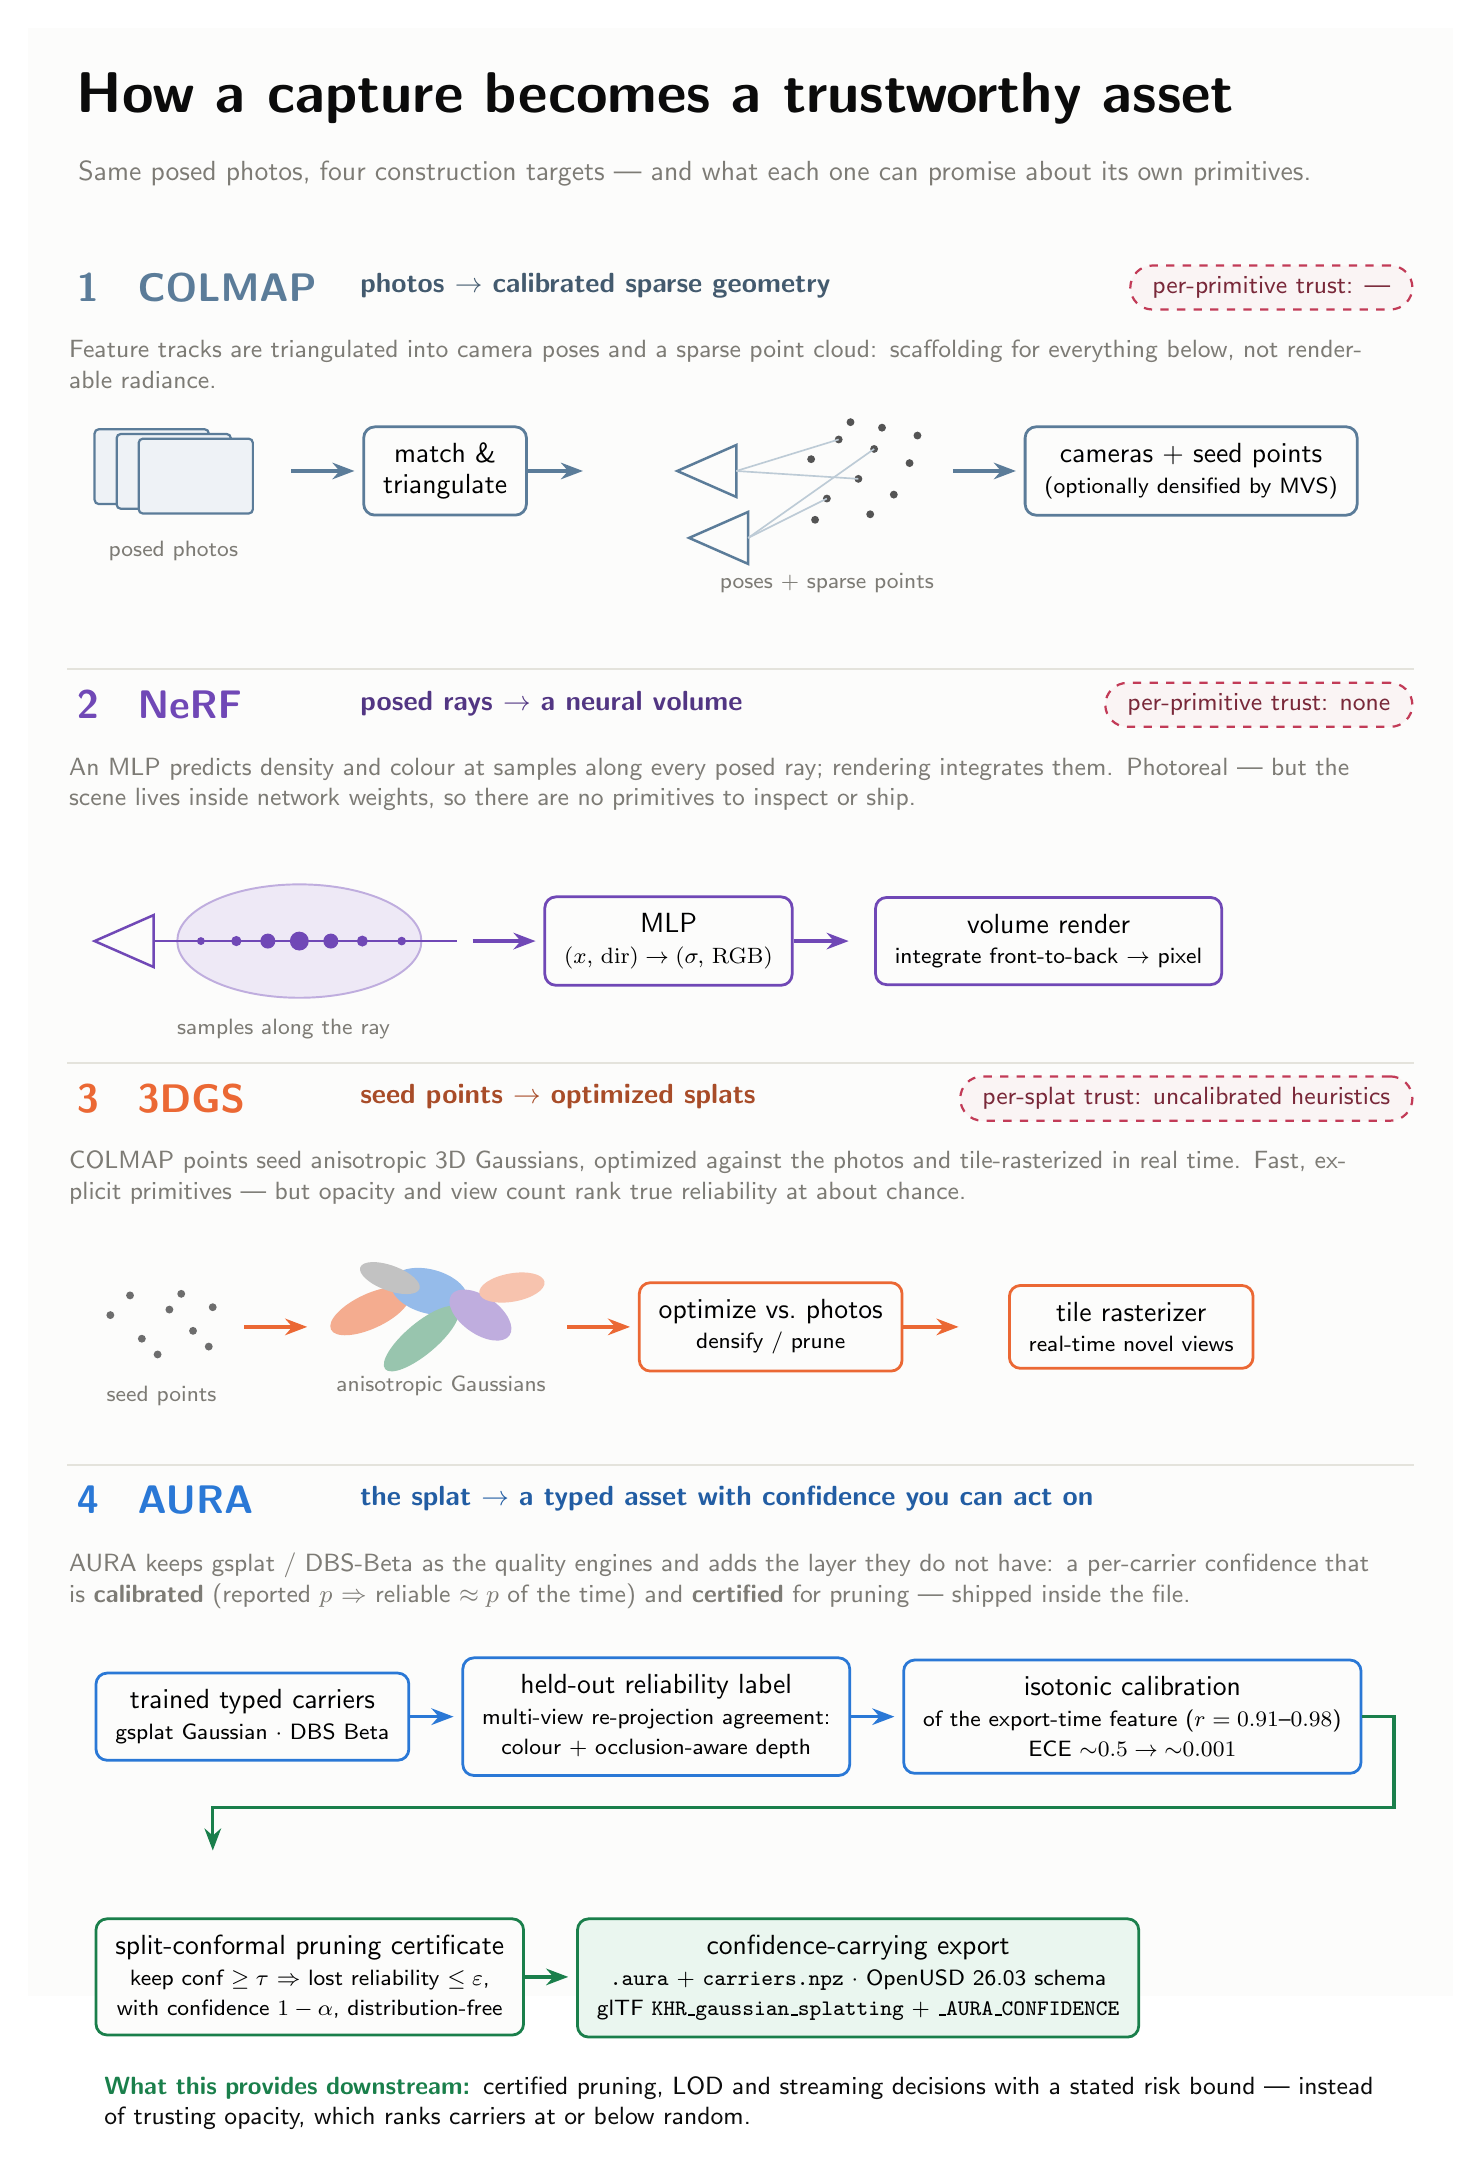
\begin{tikzpicture}[
  x=1cm, y=1cm, font=\normalsize,
  chip/.style={rounded corners=4pt, draw=#1, fill=surface, line width=1.0pt,
               inner xsep=7pt, inner ysep=6pt, align=center},
  flow/.style={-{Stealth[length=2.8mm]}, line width=1.2pt, color=#1},
  tag/.style={font=\bfseries\Large, color=#1},
  desc/.style={color=muted, font=\small, align=left, text width=16.6cm,
               inner xsep=0pt},
  glyphlab/.style={color=muted, font=\footnotesize, align=center},
  pill/.style={rounded corners=8pt, draw=rawred, dashed, fill=rawred!4!surface,
               line width=0.8pt, inner xsep=8pt, inner ysep=4pt,
               font=\small, text=rawred!60!ink}
]

\fill[surface] (-0.5,2.4) rectangle (17.6,-22.6);

% ============================== title =====================================
\node[anchor=west, font=\bfseries\huge, color=ink] at (0,1.5) {How a capture becomes a trustworthy asset};
\node[anchor=west, font=\normalsize, color=muted, align=left, text width=16.6cm] at (0.02,0.55)
  {Same posed photos, four construction targets --- and what each one can promise about its own primitives.};

% ============================== row 1: COLMAP ==============================
\begin{scope}[shift={(0,-0.9)}]
\node[tag=colmap, anchor=west] at (0,0) {1\;\; COLMAP};
\node[anchor=west, font=\normalsize\bfseries, color=colmap!70!ink] at (3.6,0.02)
  {photos $\rightarrow$ calibrated sparse geometry};
\node[pill, anchor=east] at (17.1,0) {per-primitive trust: ---};
\node[desc, anchor=north west] at (0.02,-0.55)
  {Feature tracks are triangulated into camera poses and a sparse point cloud: scaffolding for everything below, not renderable radiance.};

\begin{scope}[shift={(0.35,-2.75)}]
  \foreach \i/\dx in {0/0, 1/0.28, 2/0.56}{
    \draw[draw=colmap, fill=colmapbg, line width=0.8pt, rounded corners=1.5pt]
      (\dx,-\i*0.06) rectangle ++(1.45,0.95);
  }
  \node[glyphlab] at (1.0,-0.6) {posed photos};
  \draw[flow=colmap] (2.5,0.42) -- (3.3,0.42);
  \node[chip=colmap, anchor=west] (m) at (3.4,0.42) {match \&\\[-1pt]triangulate};
  \draw[flow=colmap] (m.east) -- ++(0.7,0);
  \begin{scope}[shift={(7.4,0.42)}]
    \draw[colmap, line width=0.9pt] (0,0) -- (0.75,0.33) -- (0.75,-0.33) -- cycle;
    \draw[colmap, line width=0.9pt] (0.15,-0.85) -- (0.9,-0.52) -- (0.9,-1.18) -- cycle;
    \foreach \p in {(1.7,0.15),(2.05,0.4),(2.3,-0.1),(1.9,-0.35),(2.5,0.28),(2.75,-0.3),(2.2,0.62),(2.6,0.55),(1.75,-0.62),(2.45,-0.55),(2.95,0.1),(3.05,0.45)}
      \fill[ink!70] \p circle (0.05);
    \draw[colmap!40, line width=0.6pt] (0.75,0) -- (2.05,0.4);
    \draw[colmap!40, line width=0.6pt] (0.75,0) -- (2.3,-0.1);
    \draw[colmap!40, line width=0.6pt] (0.9,-0.85) -- (1.9,-0.35);
    \draw[colmap!40, line width=0.6pt] (0.9,-0.85) -- (2.5,0.28);
    \node[glyphlab] at (1.9,-1.42) {poses + sparse points};
  \end{scope}
  \draw[flow=colmap] (10.9,0.42) -- (11.7,0.42);
  \node[chip=colmap, anchor=west] at (11.8,0.42) {cameras + seed points\\[-1pt]{\footnotesize (optionally densified by MVS)}};
\end{scope}
\end{scope}

% ============================== row 2: NeRF ================================
\begin{scope}[shift={(0,-6.2)}]
\node[tag=nerf, anchor=west] at (0,0) {2\;\; NeRF};
\node[anchor=west, font=\normalsize\bfseries, color=nerf!70!ink] at (3.6,0.02)
  {posed rays $\rightarrow$ a neural volume};
\node[pill, anchor=east] at (17.1,0) {per-primitive trust: none};
\node[desc, anchor=north west] at (0.02,-0.55)
  {An MLP predicts density and colour at samples along every posed ray; rendering integrates them. Photoreal --- but the scene lives inside network weights, so there are no primitives to inspect or ship.};

\begin{scope}[shift={(0.35,-3.0)}]
  \draw[nerf, line width=0.9pt] (0,0) -- (0.75,0.33) -- (0.75,-0.33) -- cycle;
  \fill[nerf!12] (2.6,0) ellipse (1.55 and 0.72);
  \draw[nerf!45, line width=0.7pt] (2.6,0) ellipse (1.55 and 0.72);
  \draw[nerf, line width=0.8pt] (0.75,0) -- (4.6,0);
  \foreach \p/\r in {1.35/0.05, 1.8/0.065, 2.2/0.095, 2.6/0.12, 3.0/0.095, 3.4/0.07, 3.9/0.055}
    \fill[nerf] (\p,0) circle (\r);
  \node[glyphlab] at (2.4,-1.12) {samples along the ray};
  \draw[flow=nerf] (4.8,0) -- (5.6,0);
  \node[chip=nerf, anchor=west] (mlp) at (5.7,0) {MLP\\[-1pt]{\footnotesize $(x,\,\mathrm{dir})\rightarrow(\sigma,\,\mathrm{RGB})$}};
  \draw[flow=nerf] (mlp.east) -- ++(0.7,0);
  \node[chip=nerf, anchor=west] at (9.9,0) {volume render\\[-1pt]{\footnotesize integrate front-to-back $\rightarrow$ pixel}};
\end{scope}
\end{scope}

% ============================== row 3: 3DGS ================================
\begin{scope}[shift={(0,-11.2)}]
\node[tag=gs, anchor=west] at (0,0) {3\;\; 3DGS};
\node[anchor=west, font=\normalsize\bfseries, color=gs!70!ink] at (3.6,0.02)
  {seed points $\rightarrow$ optimized splats};
\node[pill, anchor=east] at (17.1,0) {per-splat trust: uncalibrated heuristics};
\node[desc, anchor=north west] at (0.02,-0.55)
  {COLMAP points seed anisotropic 3D Gaussians, optimized against the photos and tile-rasterized in real time. Fast, explicit primitives --- but opacity and view count rank true reliability at about chance.};

\begin{scope}[shift={(0.35,-3.1)}]
  \foreach \p in {(0.2,0.35),(0.6,0.05),(0.45,0.6),(0.95,0.42),(0.8,-0.15),(1.25,0.15),(1.1,0.62),(1.5,0.45),(1.45,-0.05)}
    \fill[ink!60] \p circle (0.05);
  \node[glyphlab] at (0.85,-0.68) {seed points};
  \draw[flow=gs] (1.9,0.2) -- (2.7,0.2);
  \begin{scope}[shift={(3.0,0.2)}]
    \fill[gs!55, rotate around={25:(0.5,0.2)}]   (0.5,0.2)  ellipse (0.55 and 0.22);
    \fill[aura!50, rotate around={-15:(1.25,0.45)}] (1.25,0.45) ellipse (0.5 and 0.28);
    \fill[cert!45, rotate around={40:(1.15,-0.15)}] (1.15,-0.15) ellipse (0.6 and 0.2);
    \fill[nerf!45, rotate around={-35:(1.9,0.15)}]  (1.9,0.15)  ellipse (0.45 and 0.24);
    \fill[gs!40, rotate around={10:(2.3,0.5)}]  (2.3,0.5)  ellipse (0.42 and 0.18);
    \fill[ink!25, rotate around={-20:(0.75,0.62)}](0.75,0.62) ellipse (0.4 and 0.16);
    \node[glyphlab] at (1.4,-0.75) {anisotropic Gaussians};
  \end{scope}
  \draw[flow=gs] (6.0,0.2) -- (6.8,0.2);
  \node[chip=gs, anchor=west] (opt) at (6.9,0.2) {optimize vs.\ photos\\[-1pt]{\footnotesize densify / prune}};
  \draw[flow=gs] (opt.east) -- ++(0.7,0);
  \node[chip=gs, anchor=west] at (11.6,0.2) {tile rasterizer\\[-1pt]{\footnotesize real-time novel views}};
\end{scope}
\end{scope}

% ============================== row 4: AURA ================================
\begin{scope}[shift={(0,-16.3)}]
\node[tag=aura, anchor=west] at (0,0) {4\;\; AURA};
\node[anchor=west, font=\normalsize\bfseries, color=aura!75!ink] at (3.6,0.02)
  {the splat $\rightarrow$ a typed asset with confidence you can act on};
\node[desc, anchor=north west] at (0.02,-0.55)
  {AURA keeps gsplat / DBS-Beta as the quality engines and adds the layer they do not have: a per-carrier confidence that is \textbf{calibrated} (reported $p$ $\Rightarrow$ reliable $\approx p$ of the time) and \textbf{certified} for pruning --- shipped inside the file.};

\begin{scope}[shift={(0.35,-2.75)}]
  \node[chip=aura, anchor=west] (car) at (0,0)
    {trained typed carriers\\[-1pt]{\footnotesize gsplat Gaussian $\cdot$ DBS Beta}};
  \draw[flow=aura] (car.east) -- ++(0.55,0);
  \node[chip=aura, anchor=west] (lab) at ($(car.east)+(0.65,0)$)
    {held-out reliability label\\[-1pt]{\footnotesize multi-view re-projection agreement:}\\[-1pt]{\footnotesize colour + occlusion-aware depth}};
  \draw[flow=aura] (lab.east) -- ++(0.55,0);
  \node[chip=aura, anchor=west] (cal) at ($(lab.east)+(0.65,0)$)
    {isotonic calibration\\[-1pt]{\footnotesize of the export-time feature ($r=0.91$--$0.98$)}\\[-1pt]{\footnotesize ECE ${\sim}0.5\rightarrow{\sim}0.001$}};

  % wrap the chain onto a second line
  \draw[flow=cert] (cal.east) -- ++(0.4,0) -- ++(0,-1.15) -- ++(-15.0,0) -- ++(0,-0.55);
  \node[chip=cert, anchor=north west] (crt) at (0,-2.55)
    {split-conformal pruning certificate\\[-1pt]{\footnotesize keep conf $\geq\tau$ $\Rightarrow$ lost reliability $\leq\varepsilon$,}\\[-1pt]{\footnotesize with confidence $1-\alpha$, distribution-free}};
  \draw[flow=cert] (crt.east) -- ++(0.55,0);
  \node[chip=cert, anchor=north west, fill=certbg] (exp) at ($(crt.north east)+(0.65,0)$)
    {confidence-carrying export\\[-1pt]{\footnotesize \texttt{.aura} + \texttt{carriers.npz} $\cdot$ OpenUSD 26.03 schema}\\[-1pt]{\footnotesize glTF \texttt{KHR\_gaussian\_splatting} + \texttt{\_AURA\_CONFIDENCE}}};

  \node[anchor=north west, color=ink, font=\small, align=left, text width=16.4cm] at (0,-4.45)
    {{\color{cert}\textbf{What this provides downstream:}} certified pruning, LOD and streaming decisions with a stated risk bound --- instead of trusting opacity, which ranks carriers at or below random.};
\end{scope}
\end{scope}

% row separators
\foreach \y in {-5.75, -10.75, -15.85}
  \draw[grid, line width=0.7pt] (0,\y) -- (17.1,\y);

\end{tikzpicture}
\end{document}
